%\documentclass[14pt]{beamer}
\documentclass{beamer}

\usetheme{Copenhagen}
% \usetheme{Boadilla}
% \usecolortheme{beaver}
\setbeamercolor{alerted text}{fg=orange}
\setbeamercolor{background canvas}{bg=white}
\setbeamercolor{block body alerted}{bg=normal text.bg!90!black}
\setbeamercolor{block body}{bg=normal text.bg!90!black}
\setbeamercolor{block body example}{bg=normal text.bg!90!black}
\setbeamercolor{block title alerted}{use={normal text,alerted text},fg=alerted text.fg!75!normal text.fg,bg=normal text.bg!75!black}
\setbeamercolor{block title}{bg=blue}
\setbeamercolor{block title example}{use={normal text,example text},fg=example text.fg!75!normal text.fg,bg=normal text.bg!75!black}
\setbeamercolor{fine separation line}{}
\setbeamercolor{frametitle}{fg=white}
\setbeamercolor{item projected}{fg=white}
\setbeamercolor{normal text}{bg=white,fg=black}
\setbeamercolor{palette sidebar primary}{use=normal text,fg=normal text.fg}
\setbeamercolor{palette sidebar quaternary}{use=structure,fg=structure.fg}
\setbeamercolor{palette sidebar secondary}{use=structure,fg=structure.fg}
\setbeamercolor{palette sidebar tertiary}{use=normal text,fg=normal text.fg}
\setbeamercolor{section in sidebar}{fg=brown}
\setbeamercolor{section in sidebar shaded}{fg=grey}
\setbeamercolor{separation line}{}
\setbeamercolor{sidebar}{bg=red}
\setbeamercolor{sidebar}{parent=palette primary}
\setbeamercolor{structure}{bg=black, fg=white!30!blue!60!green}
\setbeamercolor{subsection in sidebar}{fg=brown}
\setbeamercolor{subsection in sidebar shaded}{fg=grey}
\setbeamercolor{title}{fg=white}
\setbeamercolor{titlelike}{fg=white}

% Szép kék
% \setbeamercolor{structure}{bg=black, fg=white!10!green!40!blue}

\frenchspacing

% Language packages
\usepackage[utf8]{inputenc}
\usepackage[T1]{fontenc}
\usepackage[magyar]{babel}

% AMS
\usepackage{amssymb,amsmath}

% Graphic packages
\usepackage{graphicx}

% Syntax highlighting
\usepackage{listings}

\usepackage{tikz}

%\begin{figure}[htb]
%\begin{center}
%	\includegraphics[scale=0.4]{ps_times.png}
%\end{center}
%\end{figure}

\usefonttheme{professionalfonts} % using non standard fonts for beamer
\usefonttheme{serif} % default family is serif
\usepackage{tgbonum}

% ==============
\begin{document}
% ==============

\title[Szürkeárnyalatos képek automatikus színezése]{Szürkeárnyalatos képek automatikus színezése gépi tanulási módszerekkel}
\author[Molnár Fanni]{\textbf{Készítette:} Molnár Fanni \\ \medskip \textbf{Témavezető:} Piller Imre}
\institute[]{Miskolci Egyetem}
\date{2022. június 9.}

% --------------------
\frame{\titlepage}

% --------------------
\begin{frame}[fragile]
\frametitle{Bevezetés}
A dolgozat során a szürkeárnyalatos képek kiszínezését vizsgáltam a Python eszközkészletének a segítségével.

\bigskip

A képek kiszínezése két problémakörre osztható:
\begin{itemize}
    \item Az összefüggő, azonos színű részek meghatározása.
    \item Az összefüggő részek kiszínezése.
\end{itemize}
\end{frame}

% --------------------
\begin{frame}[fragile]
\frametitle{K-means klaszterezés}
A klaszterezés célja, hogy egy adathalmazt klaszterekre ossza fel méghozzá úgy, hogy a klaszterezési kritérium optimális legyen.

\bigskip

A K-means módszer:
\begin{itemize}
    \item Az egyik legelterjedtebb módszer
    \item Könnyen megvalósítható
    \item Gyors, iteratív módszer
\end{itemize}
\end{frame}

% --------------------
\begin{frame}[fragile]
\frametitle{Optimális klaszterszám meghatározása}

\begin{itemize}
    \item Silhouette módszer
    \item Davies-Bouldin módszer
    \item Calinski-Harabasz módszer
    \item Elbow módszer
\end{itemize}

\begin{figure}[!tbp]
  \centering
  \begin{minipage}[b]{0.7\textwidth}
      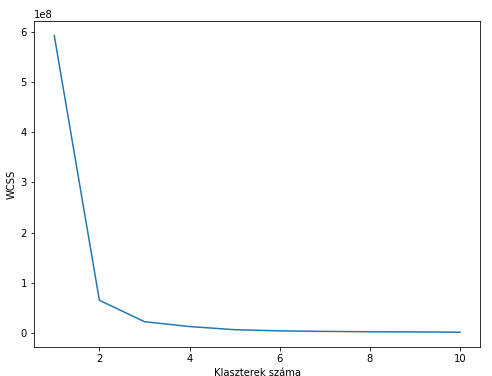
\includegraphics[width=\textwidth]{images/elbow_grayscale.png}
  \end{minipage}
\end{figure}

\end{frame}

% --------------------
\begin{frame}[fragile]
\frametitle{K-means klaszterezés intenzitás alapján}
\begin{figure}[!tbp]
  \centering
  \begin{minipage}[b]{0.7\textwidth}
      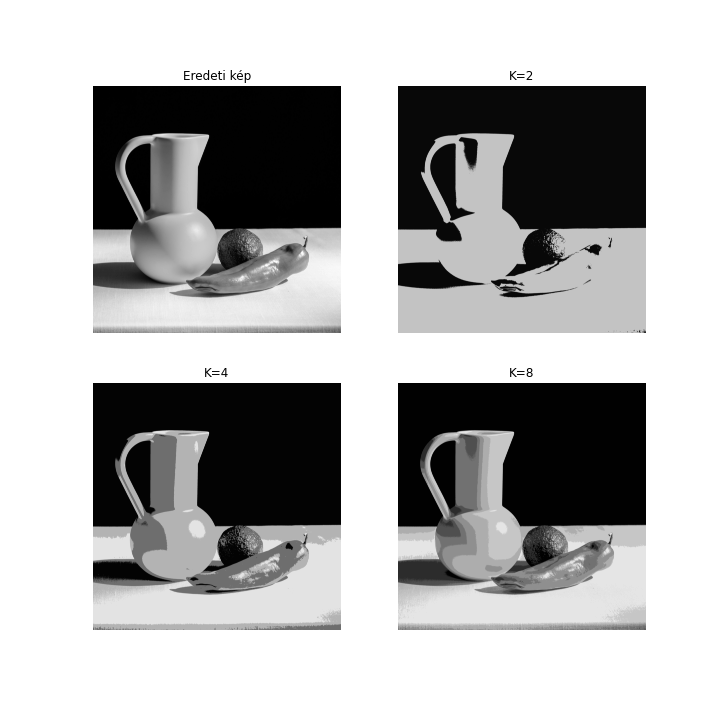
\includegraphics[width=\textwidth]{images/kmeans_grayscale.png}
  \end{minipage}
\end{figure}
\end{frame}

% --------------------
\begin{frame}[fragile]
\frametitle{K-means klaszterezés textúra alapján}
\begin{figure}[!tbp]
  \centering
  \begin{minipage}[b]{0.55\textwidth}
    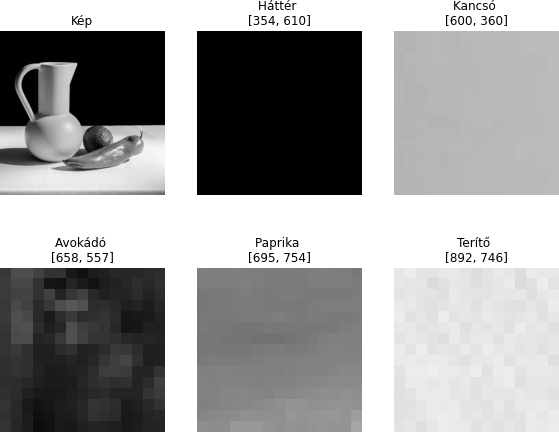
\includegraphics[width=\textwidth]{images/window_example.png}
  \end{minipage}
  \hfill
  \begin{minipage}[b]{0.4\textwidth}
    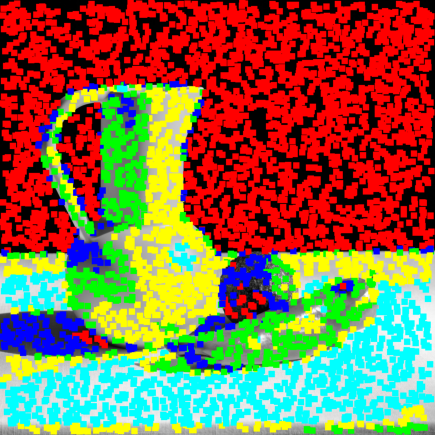
\includegraphics[width=\textwidth]{images/window_colorized.png}
  \end{minipage}
\end{figure}
\end{frame}

% --------------------
\begin{frame}[fragile]
\frametitle{KNN osztályozás}
\begin{figure}[!tbp]
  \centering
  \begin{minipage}[b]{1\textwidth}
      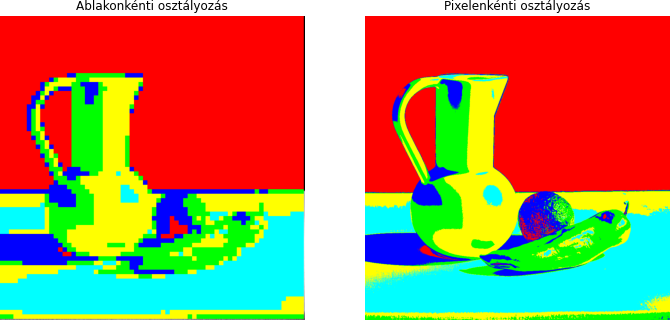
\includegraphics[width=\textwidth]{images/window_pixel_segmentation.png}
  \end{minipage}
\end{figure}
\end{frame}

% --------------------
\begin{frame}[fragile]
\frametitle{Szuperpixel alapú módszerek}

\begin{figure}[!tbp]
  \centering
  \begin{minipage}[b]{0.65\textwidth}
    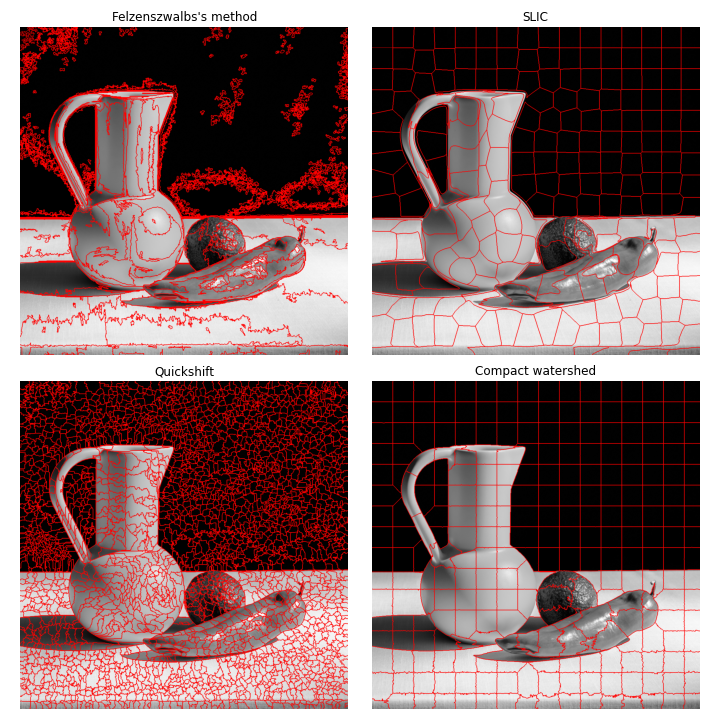
\includegraphics[width=\textwidth]{images/superpixel_example.png}
  \end{minipage}
\end{figure}

\end{frame}

% --------------------
\begin{frame}[fragile]
\frametitle{Szürkeárnyalatos képek kiszínezése}
A szürkeárnyalatos képek kiszínezése az árnyalatok megjelenítésével. A minél jobb eredmény elérésének érdekében az RGB és HSV színterekben is megvizsgáltam a problémát.
\begin{figure}[!tbp]
  \centering
  \begin{minipage}[b]{0.45\textwidth}
    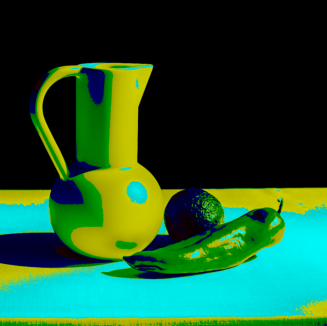
\includegraphics[width=\textwidth]{images/colorized_rgb.png}
  \end{minipage}
  \hfill
  \begin{minipage}[b]{0.45\textwidth}
    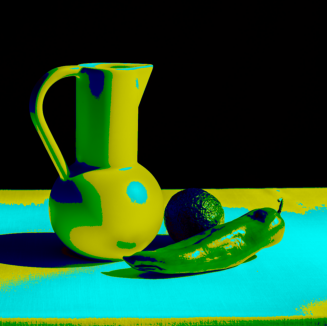
\includegraphics[width=\textwidth]{images/colorized_hsv.png}
  \end{minipage}
\end{figure}
\end{frame}

% --------------------
\begin{frame}[fragile]
\frametitle{Képek színének visszabecslése}
A színek visszabecslésére CNN modellt használok. A modell általam megadott, 13 kategória (szín) közül választja ki a becsült értéket.

\begin{figure}[!tbp]
  \centering
  \begin{minipage}[b]{0.58\textwidth}
    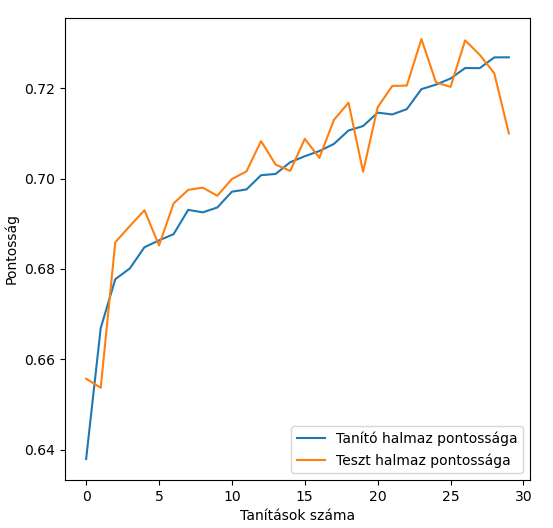
\includegraphics[width=\textwidth]{images/cnn_accuracy.png}
  \end{minipage}
\end{figure}
\end{frame}

% --------------------
\begin{frame}[fragile]
\frametitle{Eredmény - K-means}

\begin{figure}[!tbp]
  \centering
  \begin{minipage}[b]{0.9\textwidth}
    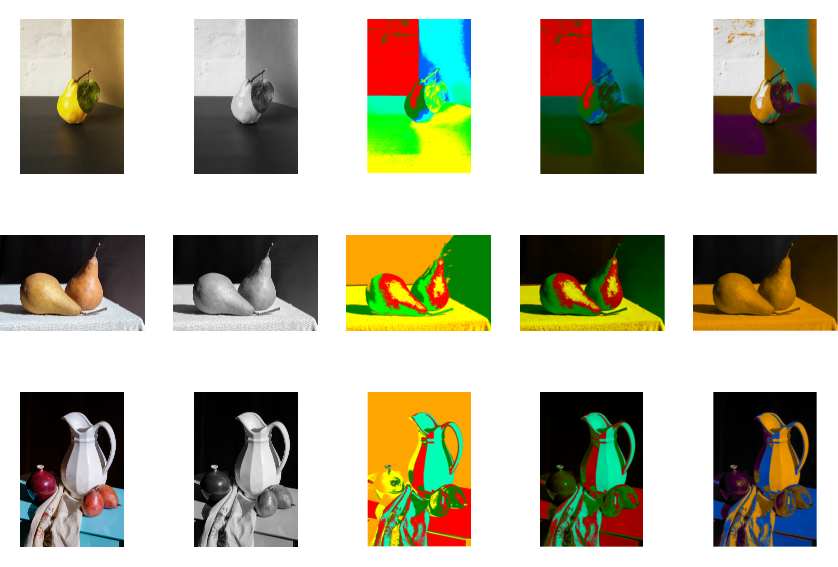
\includegraphics[width=\textwidth]{images/result_all_kmeans.png}
  \end{minipage}
\end{figure}

\end{frame}

% --------------------
\begin{frame}[fragile]
\frametitle{Eredmény - Szuperpixel}

\begin{figure}[!tbp]
  \centering
  \begin{minipage}[b]{0.8\textwidth}
    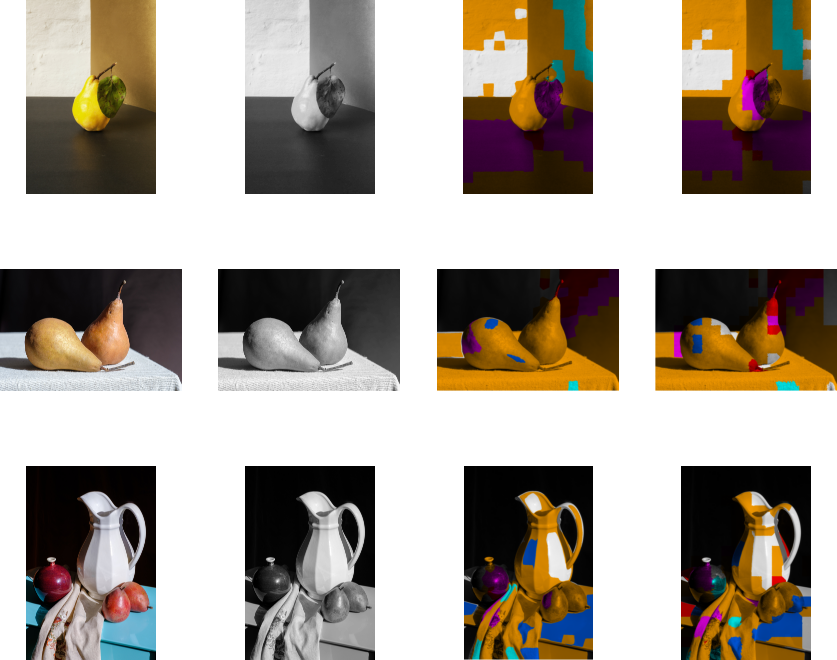
\includegraphics[width=\textwidth]{images/result_all_superpixel.png}
  \end{minipage}
\end{figure}

\end{frame}

% --------------------
\begin{frame}[fragile]
\frametitle{Összegzés}
\begin{itemize}
	\item A szürkeárnyalatos képekből visszanyerni a kép eredeti színeit az nem egy egyszerű feladat abban az esetben, ha nincsen a programnak kiindulási alapja.
    \item Szürkeárnyalatos képek szegmentálására nem a K-means a legmegfelelőbb módszer.
    \item Vissza színezés esetén a HSV színtér használata sokkal egyszerűbb, mint az RGB színtéré.
\end{itemize}

\end{frame}

% --------------------
\begin{frame}[fragile]
\frametitle{Felhasznált irodalmak}

\begin{itemize}
	\item Python.org. Packaging python projects. https://packaging.python.org/en/latest/tutorials/
    packaging-projects/
    \item OpenCV. K-means clustering in opencv. https://docs.opencv.org/4.x/d1/d5c/
    tutorial\_py\_kmeans\_opencv.html
    \item Comparison of segmentation and superpixel algorithms. https://\mbox{scikit-image}.org/docs/stable/
    \mbox{auto\_examples}/segmentation/
    plot\_segmentations.html
    \item Khushbu Raval, Ravi Shukla, and Ankit K Shah. Color image segmentation using fcm clustering technique in rgb, l* a* b, hsv, yiq color spaces. Eur. J. Adv. Eng. Technol, 4(3):194U200, 2017.
\end{itemize}

\end{frame}

% --------------------
\begin{frame}[fragile]
\frametitle{\ }

\begin{center}

    \Large

    \textbf{Köszönöm szépen a figyelmet!}

    \bigskip

\end{center}

\end{frame}

\end{document}

